\documentclass{beamer}
\usetheme{metropolis}
\usepackage{graphicx}
\usepackage{subfig}
\title{Safe Return Doubtful: Week 2 part I}
\date{\today}
\author{Jordan Hanson}
\institute{Whittier College Department of Physics and Astronomy}

\begin{document}
\maketitle

\section{Summary}

\begin{frame}{Summary}
\begin{enumerate}
\item A few words about the reading, the next reading quiz
\item Warm-up: work with friction, mass, and distance.
\begin{itemize}
\item $W = \mu m g d$
\item \textbf{Now in 2D! Because navigation takes place in two-dimensions}
\item In the future, we'll put this together with calories
\item \textbf{3D: terrain (different frictions) and \textit{elevation}}
\end{itemize}
\item \textbf{Lecture: My expeditions to Moore's Bay, Antarctica}
\end{enumerate}
\end{frame}

\section{Warm-up}

\begin{frame}{Warm-up}
\small
Moving a load of food and equipment against friction:
\begin{equation}
W = \mu m g d
\end{equation}
\begin{itemize}
\item Suppose we are pulling a load of gear with a tractor across sand.  The gear has mass $m = 300$ kg, the distance is $d = 12$ km, and $g = 9.81$ m/s$^2$.  If the friction coefficient is 0.2, how much work (in Watts) does the tractor do?
\item Did you know that there are 7600 kcal of energy in one liter of gasoline?  Convert this to megajoules.
\item How many liters of gas is required to move the load?
\item Assuming that the tractor also burns 0.4 liters each kilometer just to move itself.  How many liters is this, if we go 12 km?
\item How many liters of gasoline are required, in total?
\end{itemize}
\end{frame}

\section{Motion (navigation) in 2D}

\begin{frame}{Motion (navigation) in 2D}
\begin{figure}
\centering
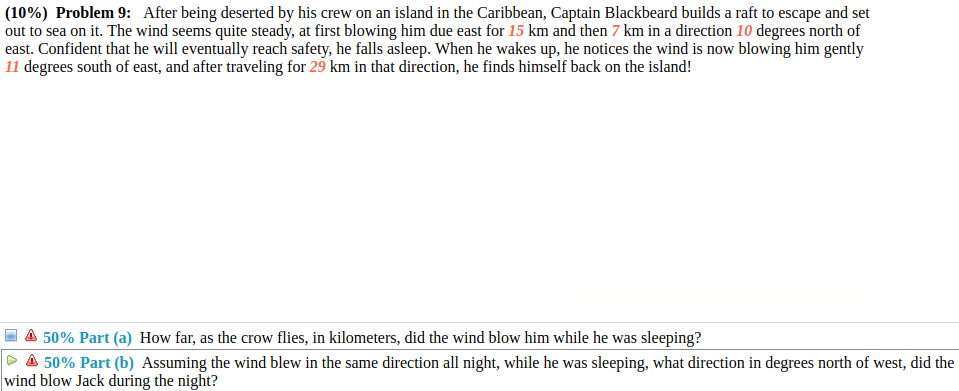
\includegraphics[width=0.9\textwidth]{navigationExample.png}
\caption{\label{fig:navEx} This is an example problem from introductory physics course.  To solve the problem, we need to understand a piece of math called a \textit{vector.}}
\end{figure}
\end{frame}

\begin{frame}{Coordinates and Vectors - Applications: Displacement}
Navigation in the film The Hunt for Red October:
\url{https://youtu.be/4unk6siO-tI}
\end{frame}

\begin{frame}{Coordinates and Vectors - Scalars, Vectors}
Physics requires \alert{mathematical objects} to build equations that capture the behavior of nature.  Two examples of such objects are \alert{scalar} and \alert{vector} quantities.  Each type of object obeys similar but different rules.
\begin{enumerate}
\item Scalar quantities
\begin{itemize}
\item mass: $m_1+(m_2+m_3) = (m_1+m_2)+m_3$
\item speed: $v_1(v_2+v_3) = v_1v_2+v_1v_3$
\item charge: $q_1 \left(\frac{1}{q_1}\right) = 1$, $q_1(0) = 0$
\end{itemize}
\item Vector quantities
\begin{itemize}
\item displacement: $\Delta x = \vec{x}_f - \vec{x}_i$
\item velocity: $\vec{v}_1 + (\vec{v}_2+\vec{v}_3) = (\vec{v}_1 + \vec{v}_2)+\vec{v}_3$
\end{itemize}
\end{enumerate}
\textbf{Professor: show how to break into components, connection to trigonometry.}
\end{frame}

\begin{frame}{Coordinates and Vectors - Scalars, Vectors (Chapters 2.1-2.2)}
A vector may be expressed as \textit{a list of scalars}: $\vec{v} = (4,2)$ (a vector with two \textit{components}), $\vec{u} = (3,4,5)$ (three \textit{components}).  Now, we know how to add and subtract scalars.  How do we add and subtract vectors? \\
\vspace{0.5cm}
What is\\
$(1,3,8)+$\\ $(0,2,1)$? \\
Answer: $(1,5,9)$ \\
\vspace{0.5cm}
In other words, when adding vectors, we add them component by component. \textbf{Professor: work several examples.}
\end{frame}

\begin{frame}{Coordinates and Vectors - Scalars, Vectors (Chapters 2.1-2.2)}
How do we subtract vectors? In the same fashion:\\
\vspace{0.5cm}
What is\\
$(1,3,8)-$\\ $(0,2,1)$? \\
Answer: $(1,1,7)$ \\
\vspace{0.5cm}
In other words, when subtracting vectors, we subtract them component by component. \textbf{Professor: work several examples.}
\end{frame}

\begin{frame}{Coordinates and Vectors - Coordinates (Chapters 2.1-2.2)}
\small
The components of a vector may describe quantities in a \alert{coordinate system}, such as \textit{Cartesian coordinates} - after Ren\'e Descartes.  Vectors in the 3D Cartesian coordinate system (x,y,z) may be written in the following notation:
\\
\vspace{0.2cm}
$\boxed{\vec{v} = a\hat{i} + b\hat{j} + c\hat{k}}$
\\
\begin{itemize}
\item a: The amount in the +x-direction, $\hat{i}$: a vector of length 1, in the +x-direction
\item b: The amount in the +y-direction, $\hat{j}$: a vector of length 1, in the +y-direction
\item c: The amount in the +z-direction, $\hat{k}$: a vector of length 1, in the +z-direction
\end{itemize}
\end{frame}

\begin{frame}{Coordinates and Vectors - Vectors (Chapters 2.1-2.2)}
\begin{figure}
\centering
\subfloat[\label{fig:twovectors_a}]{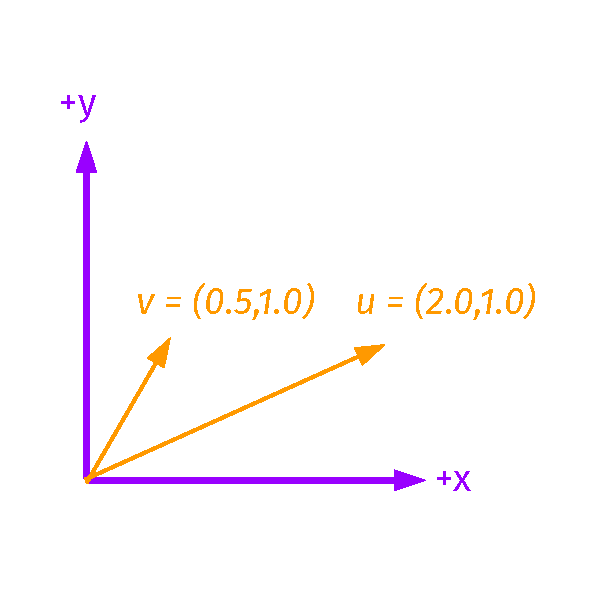
\includegraphics[width=0.45\textwidth,trim=1cm 1cm 1cm 1cm,clip=true]{figures/Vectors1.pdf}}
\subfloat[\label{fig:twovectors_b}]{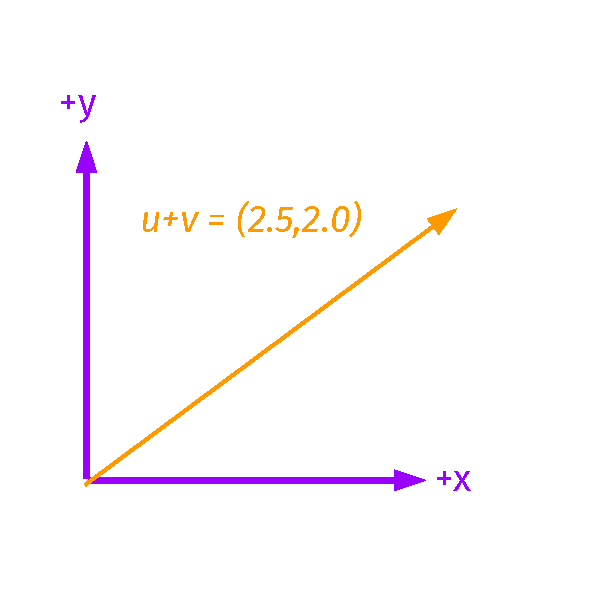
\includegraphics[width=0.45\textwidth,trim=1cm 1cm 1cm 1cm,clip=true]{figures/Vectors2.pdf}}
\caption{\label{fig:twovectors} (a) Two vectors in a two-dimensional Cartesian coordinate system: $\vec{u} = 0.5\hat{i}+1.0\hat{j}$ and $\vec{v} = 2.0\hat{i}+1.0\hat{j}$.  (b) What is $\vec{u}+\vec{v}$?  Adding components: $\vec{u}+\vec{v} = 2.5\hat{i}+2.0\hat{j}$.}
\end{figure}
\end{frame}

\begin{frame}{Coordinates and Vectors - Vectors (Chapters 2.1-2.2)}
\begin{figure}
\centering
\subfloat[\label{fig:twovectors_c}]{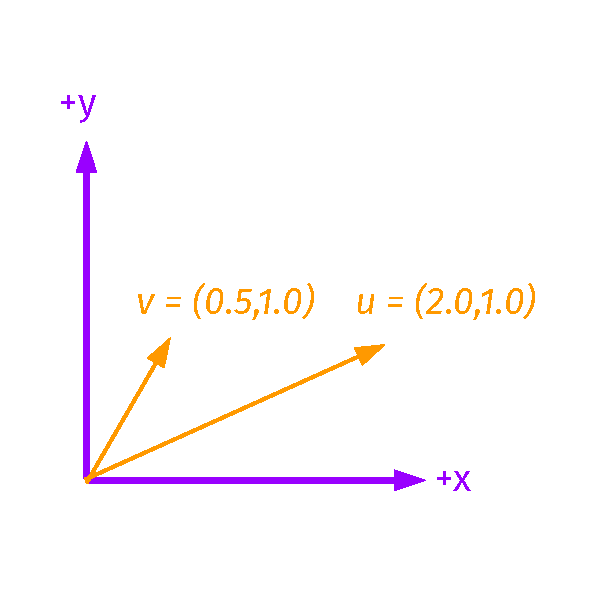
\includegraphics[width=0.45\textwidth,trim=1cm 1cm 1cm 1cm,clip=true]{figures/Vectors1.pdf}}
\subfloat[\label{fig:twovectors_d}]{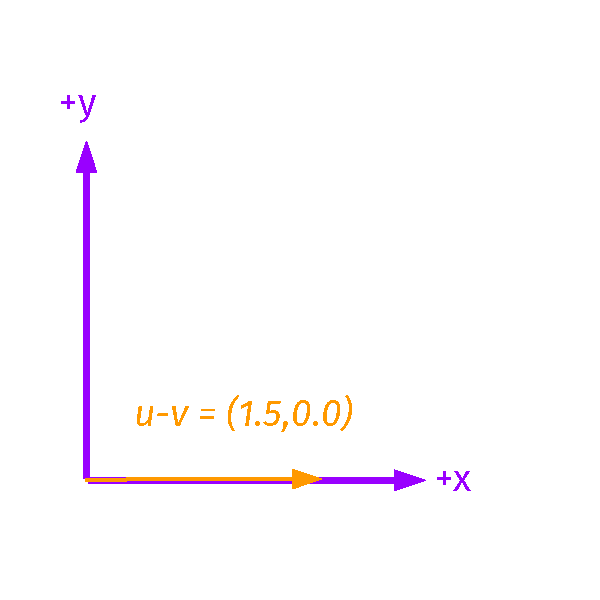
\includegraphics[width=0.45\textwidth,trim=1cm 1cm 1cm 1cm,clip=true]{figures/Vectors3.pdf}}
\caption{\label{fig:twovectors2} (a) Two vectors in a two-dimensional Cartesian coordinate system: $\vec{u} = 0.5\hat{i}+1.0\hat{j}$ and $\vec{v} = 2.0\hat{i}+1.0\hat{j}$.  (b) What is $\vec{u}-\vec{v}$?  Subtracting components: $\vec{u}-\vec{v} = 1.5\hat{i}+0.0\hat{j}$.}
\end{figure}
\end{frame}

\begin{frame}{Coordinates and Vectors - Vectors (Chapters 2.1-2.2)}
\begin{figure}
\centering
\subfloat[\label{fig:twovectors_e}]{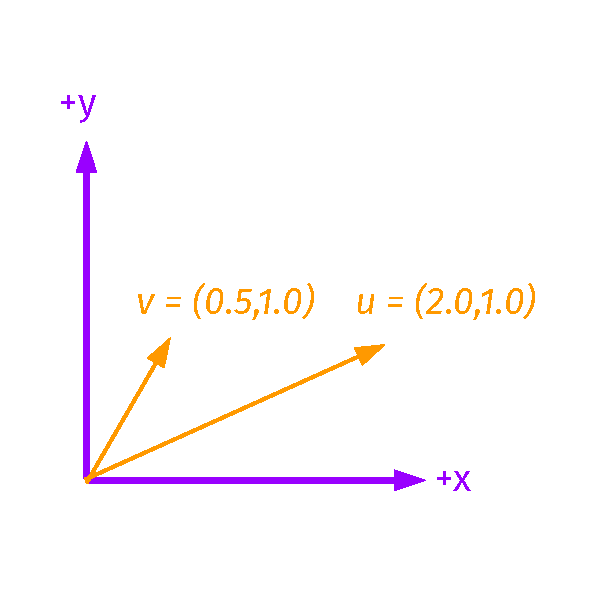
\includegraphics[width=0.45\textwidth,trim=1cm 1cm 1cm 1cm,clip=true]{figures/Vectors1.pdf}}
\subfloat[\label{fig:twovectors_f}]{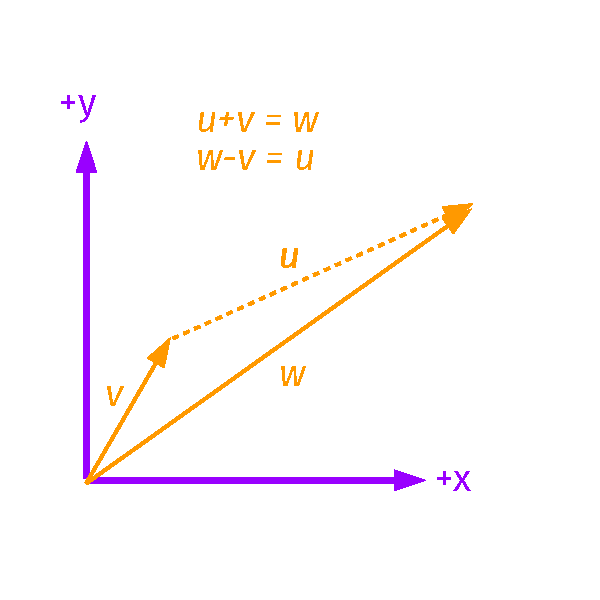
\includegraphics[width=0.45\textwidth,trim=1cm 1cm 1cm 1cm,clip=true]{figures/Vectors4.pdf}}
\caption{\label{fig:twovectors3} (a) Two vectors in a two-dimensional Cartesian coordinate system: $\vec{u} = 0.5\hat{i}+1.0\hat{j}$ and $\vec{v} = 2.0\hat{i}+1.0\hat{j}$.  (b) To compute $\vec{w}-\vec{v}$, arrange the vectors to get a sense of the result, $\vec{u}$.}
\end{figure}
\end{frame}

\begin{frame}{Coordinates and Vectors - Dot Product (Chapters 2.1-2.2)}
The \textit{length} or \textit{norm} of a vector $\vec{v} = a\hat{i}+b\hat{j}$ is $|\vec{v}| = \sqrt{a^2+b^2}$.\\
\begin{figure}
\centering
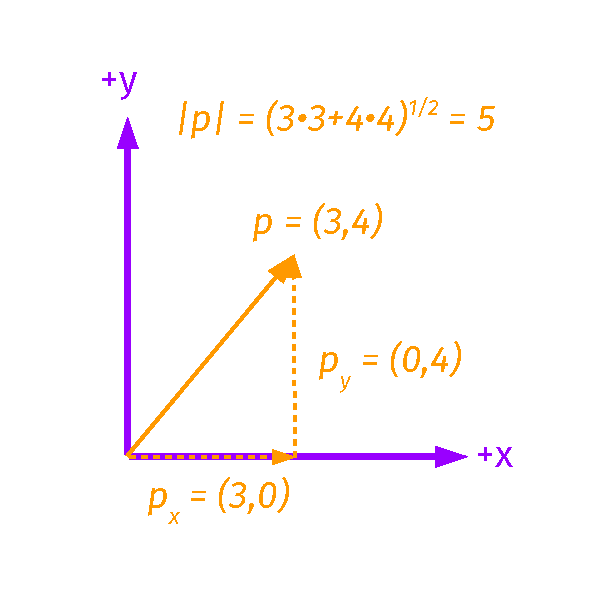
\includegraphics[width=0.5\textwidth,trim=1cm 1cm 1cm 1cm,clip=true]{figures/Vectors7.pdf}
\caption{\label{fig:twovectors6} Computing the norm of a vector $\vec{p}$.}
\end{figure}
\end{frame}

\begin{frame}{Coordinates and Vectors - Dot Product (Chapters 2.1-2.2)}
\small
An object moves 10 km at $\theta = 60^{\circ}$ North of East.  How far East did it go, and how far North did it go?
\begin{itemize}
\item Break the \textit{displacement} vector into North part and East part by drawing a triangle.  One leg is the East part and one leg is the North part.
\item Use sine and cosine, plus the angle, to find the length of each triangle leg.
\end{itemize}
\end{frame}

\begin{frame}{Coordinates and Vectors - Dislacement (Chapters 2.1-2.2)}
We define the \textit{position} of an object as a vector locating it in a given coordinate system.  The scalar \textit{distance} is the norm of the position vector, that is, the distance to to the origin. \\
\vspace{0.5cm}
Now we can introduce the concept of \alert{dislacement}: a vector describing a movement of an object.
\end{frame}

\begin{frame}{Coordinates and Vectors - Displacement (Chapters 2.1-2.2)}
\begin{figure}
\centering
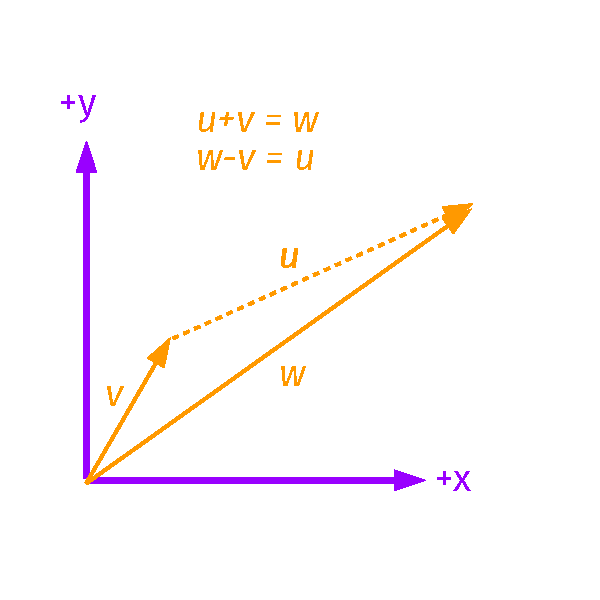
\includegraphics[width=0.52\textwidth]{figures/Vectors4.pdf}
\caption{\label{fig:displacement} Suppose an object moves from position $\vec{v}$ to $\vec{w}$.  In this case, the \alert{displacement} is $\vec{u}$. \textbf{Thus, the final position is the initial position, plus the displacement.}}
\end{figure}
\end{frame}

\begin{frame}{Coordinates and Vectors - Computer demonstration}
Download the Java applet (you may need to update Java): \\
\url{https://phet.colorado.edu/en/simulation/vector-addition}
\end{frame}

\begin{frame}{Coordinates and Vectors - Average Velocity  (Chapter 2.3)}
\alert{Average velocity} is the ratio of the \alert{displacement} to the elapsed time.\\
\begin{equation}
\boxed{\vec{v}_{\rm avg} = \frac{\Delta \vec{x}}{\Delta t}}
\end{equation}
The \textit{average speed} is the norm of the average velocity:
\begin{equation}
\boxed{v_{\rm avg} = \frac{|\Delta \vec{x}|}{\Delta t}}
\end{equation}
If the motion is in one dimension, then the average speed is
\begin{equation}
v_{\rm avg} = \frac{x_{\rm f} - x_{\rm i}}{t_{\rm f} - t_{\rm i}}
\end{equation}
\end{frame}

\begin{frame}{Coordinates and Vectors - Average Velocity (Chapter 2.3)}
\begin{figure}
\centering
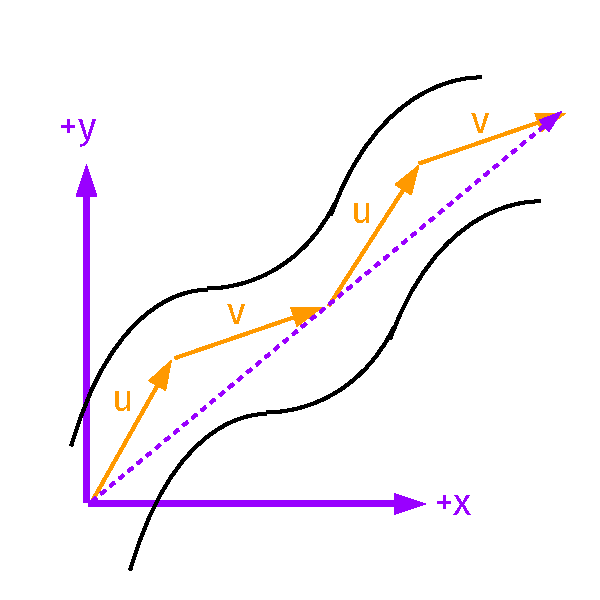
\includegraphics[width=0.52\textwidth]{figures/AveVelocity.pdf}
\caption{\label{fig:avevel} A Formula-1 driver keeps his car on the track by following a path approximated by the position vectors $u$, $v$, $u$, and $v$.  The dashed arrow represents the total displacement.}
\end{figure}
\end{frame}

\begin{frame}{Motion (navigation) in 2D}
\begin{figure}
\centering
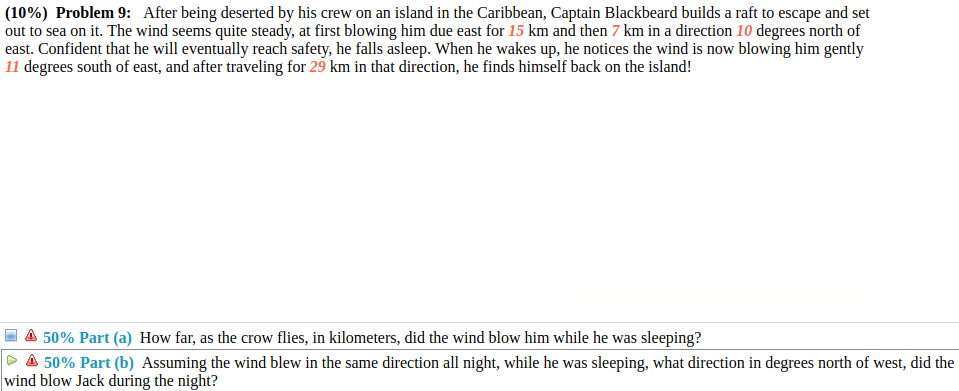
\includegraphics[width=0.9\textwidth]{navigationExample.png}
\caption{\label{fig:navEx} This is an example problem from introductory physics course.  To solve the problem, we need to understand a piece of math called a \textit{vector.}}
\end{figure}
\end{frame}

\section{The Story of ARIANNA, part I}

\end{document}
